\documentclass[a4paper, 10pt, 
               numbers=noenddot, toc=graduated,
               headsepline=true, footsepline=true,
               twoside=false, titlepage=true, 
               bibliography=totoc]{scrartcl}



\usepackage[a4paper, top = 2.5cm,
  	bottom = 2.0cm,
    left   = 2.0cm,
    right  = 2.0cm]{geometry}

\usepackage{graphicx}
\usepackage{amsmath} %math package
\usepackage{amssymb}
\usepackage[font={footnotesize}, bf]{caption}
\renewcommand{\arraystretch}{1.2}
\usepackage{bm}
\usepackage{longtable}
\usepackage{lscape}
\usepackage{siunitx}	
%\usepackage{citesort} 
\usepackage{physics}

\usepackage[toc,page]{appendix}
\setlength\parindent{0pt}
\usepackage{subcaption}
\usepackage{cite} 
%\usepackage{float} 
\usepackage[utf8x]{inputenc}		% input encoding
\usepackage[ngerman]{babel} 
\captionsetup{format=plain}
\addto\captionsenglish{\renewcommand{\figurename}{Fig.}}
\addto\captionsenglish{\renewcommand{\tablename}{Tab.}}
\usepackage[T1]{fontenc}                % mathmode for font Palatino
%\usepackage[plainfootsepline ,autooneside]{scrpage2}	% header and footer for komascript
\usepackage{hyperref}
\usepackage[procnames]{listings}

\usepackage{url}
\usepackage{titling}
\usepackage{multirow}
 

\usepackage{floatrow}
% Table float box with bottom caption, box width adjusted to content
\newfloatcommand{capbtabbox}{table}[][\FBwidth]


\usepackage{array}

\makeatletter
\newcommand{\thickhline}{%
    \noalign {\ifnum 0=`}\fi \hrule height 1pt
    \futurelet \reserved@a \@xhline
}
\newcolumntype{"}{@{\hskip\tabcolsep\vrule width 1pt\hskip\tabcolsep}}
\makeatother

\newcommand{\refeqn}[1]  {Gleichung~\ref{#1}}  
\newcommand{\refsec}[1]  {Abschnitt~\ref{#1}}  
%\usepackage{fancyhdr}
%\pagestyle{fancy}
%\fancyhf{}
%\fancyheadoffset{0 cm}

%\rhead{\nouppercase\rightmark}
%\lhead{\thepage}

\newif\ifinternal

\internalfalse

\newcommand*\mean[1]{\overline{#1}}

\begin{document}

\title{Bestimmung der strahlungsinduzierten Viskosit{\"a}t mit Hilfe von LAMMPS}
\author{Christian Schleich, Alexander Toifl}

\begin{center}
\huge{\thetitle} \\
\small{\theauthor, \today}
\end{center}

%\tableofcontents
\hspace{1 cm}


\section{Strahlungsinduzierte und dynamische Viskosität}

\subsection{Definitionen und Begriffe}



\begin{itemize}
	\item Definition der dynamischen Viskosität
	
	      \begin{equation}
		  \eta = \frac{\tau }{\dot{\gamma} }
	      \end{equation}
	      $\tau$ ... Schubspannung\\
	      $\dot{\gamma} $ ... Geschwindigkeitsprofil senkrecht zur Richtung in der die Schubspannung wirkt

	\item Grundidee der strahlungsinduzierten Viskosität \cite{hobler2017hpm}
	
		\begin{itemize}
			
			\item Ionenbeschuss des Targets mit bestimmter Dosis führt zur Verschiebung von Atomen (displacement).
			\item Wenn die Dosis zeitlich variiert wird mit einer gewissen Dosisrate $\dot \phi$, ergibt sich ein zeitlicher Verlauf der Anzahl der Displacements $n_\mathrm{dpa}(t)$.
			\item Folglich ergibt sich ein ortsabhängiger Nettofluss von Atomen, die zu einem veränderten Geschwindigkeitsprofil führt.
			
			\item Daher hängt die dynamische Viskosität $\eta$ von der Energiedeposition in Form der Displacements ab (orts- und dosisratenabhängig: $\eta = \eta(\bm{x}, \dot{\phi})$).
			
			\item Unter der Annahme, dass die Spannungs-Relaxation als Antwort auf eine (bspw. biaxiale) Verzerrung \textbf{nur von den Displacments} herrührt (\textit{Ist diese Annahme gerechtfertigt?}), gibt es eine orts- und dosisraten\textbf{un}abhängige Größe, die das viskose Verhalten des gesamten Targets beschreibt - die strahlungsbezogene Viskosität $\eta^{'}$.
			\begin{equation}
		  		\frac{\partial \bm{\varepsilon}}{\partial n_\mathrm{dpa} } = \frac{1}{2G} \frac{\partial \bm{\sigma}}{\partial n_\mathrm{dpa}} + \frac{1}{2 \eta^{'} }\bm \sigma
	      	\end{equation}
	      	
	      	$ \bm{\varepsilon}$ ... Verzerrungstensor\\
	      	$\bm\sigma$ ... Spannungstensor\\
	      	$G$ ... Schubspannungsmodul
			
					     
		\end{itemize}
	
	\item Definition der Strahlungsinduzierten Fluidität $H$ nach \cite{Mayr2003}
	      \begin{equation}\label{eqn:visc_mayer}
		    H = \frac 1 {\eta \dot{\phi}} = \frac 1 {\eta^{'}}\, \implies \quad \eta^{'} = \eta \dot{\phi}
	      \end{equation}  
		$\eta$ ... dynamische Viskosität mit $\left[\eta\right] = Pa \cdot s$\\
		$\eta^{'}$ ... strahlungsind. Viskosität mit $\left[\eta^{'}\right] = Pa \cdot dpa$
		
	\item Beziehung zwischen dynamischer und strahlungsinduzierter Viskosität nach nach \cite{hobler2017hpm}
	      \begin{equation}\label{eqn:visc_hobler}
		    \eta^{'} = \eta \frac{\partial n_\mathrm{dpa}}{\partial t} = \eta \frac{\partial n_\mathrm{dpa}}{\partial \phi} \dot{\phi}
	      \end{equation} 
		$ n_\mathrm{dpa}$ ... Anzahl der Displacments \\
		$\phi$ ... Implantationsdosis\\
		$\dot{\phi}$ ... Implantationsdosisrate\newline
		\textit{Wie lässt sich die Diskrepanz zwischen \refeqn{eqn:visc_mayer} und \refeqn{eqn:visc_hobler} erklären? Nehmen Mayr et al. einen linearen Zusammenhang der Form $n_\mathrm{dpa}(\phi) = k \phi$ an?}
		
		
	
\end{itemize}


\subsection{Bestimmung der strahlungsinduzierten Viskosität mittels Molekulardynamik Simulationen}

\begin{itemize}

   \item \textit{Setup der MD Simulation (Amorphisierung, Equilibrierung, ...)}
   
	\begin{itemize}
	   \item Allgemeine Informationen zum Aufschmelzen und Abkühlen (Temperatur und Druck) mit MD - Simulationen (in Ge - Dünnschichten) zur Amorphisierung des Materials finden sich in \cite{Mayr2005}. 
	   
	   \item Außerdem werden auch Werte für die strahlungsinduzierte Viskosität in Abhängigkeit der Defektdichte dpa angegeben - selbe Methode wie in \cite{Mayr2003}. 

	   \item Ebenfalls wird dies in \cite{Edler2007} beschrieben, wobei hier aber nur mech. Stressbetrachtungen gemacht werden. 
	   
	   \item In \cite{Lehnert2017} wird die in \cite{Mayr2003} erwähnte Methode auf a-Ge-Si Legierungen angewandt um mithilfe der Fluidität die Formierung von porösen Strukturen zu begründen.
	   
	\end{itemize}	   
   
   \item \textit{Wie werden Recoils eingebracht? Künstlich wie in \cite{Mayr2003}? Oder durch Ionendeposition wie beim Sputtern?}\\
In \cite{Mayr2005} wird eine zufällig orientierte Geschwindigkeit (entspricht der gewünschen Recoil-Energie) zufällig ausgewählten Atomen zugewiesen. Dabei werden unterschiedliche Randbedingungen verwendet (periodisch in alle Richtungen, periodisch in x,y und offen in z) um den Einfluss von Oberflächeneffekten zu berücksichtigen. Die 3 äußeren Lagen der Simulationsbox werden Temperatur-geregelt und pro eV kinetischer Energie werden 25 Atome simuliert um unerwünschtes Aufheizen zu vermeiden. 

   \item \textit{Wie können die Standardmethoden zur Berechnung der Viskosität von Flüssigkeiten (\refsec{sec:visc}) so abgewandelt werden, dass sich die strahlungsinduzierte Viskosität ergibt?}
   
 

\end{itemize}


\section{MD Methoden zur Bestimmung der Viskosität}\label{sec:visc}

\subsection{Non-equilibrium MD (NEMD) Simulationen}

System wird verformt (Scherung) und die resultierende Spannung wird ermittelt. 


	\subsubsection{SLLOD}
		\begin{itemize}
		 	\item Original Paper, in dem SLLOD Dynamik vorgestellt werden \cite{Evans1984}, welche für alle homogenen Körper gilt.
		 	\item Dem System wird eine Schergeschwindigkeit (shear rate) $\dot{\gamma}$ aufgezwungen. Als Folge ergibt sich ein Impulsfluss, der über die Nicht-Diagonalelemente des Spannungs- oder Drucktensors gemessen wird\cite{Tenney2010}. Die Scherviskosität ergibt sich damit zu 
				\begin{equation}
					\eta\left(\dot{\gamma}\right) = - \frac{P_{ij}}{\dot{\gamma}}
					\label{equ:sllod}
				\end{equation}
 mit $P_{ij}$ den Nicht-Diagonalelementen des Stress - Tensors. i beschreibt die Flussrichtung und j die Normalrichtung darauf. 
		 	\item Problem: Druck variiert typischerweise sehr stark in MD Simulationen, daher ist die Konvergenz eher langsam\cite{Tenney2010}.
		 	\item LAMMPS: Mit der Verwendung des \texttt{fix nvt/sllod} und \texttt{fix deform} 
				\begin{itemize}
					\item \texttt{fix nvt/sllod} startet eine NVT-Simulation mit einem Nose/Hoover Thermostat. Die Temperatur wird dabei aus der kinetischen Energie der Teilchen abzüglich der von der Scherung herrührenden kinetischen Energie berechnet. (die positionsabhängige 'Fließgeschwindigkeit' jedes Atoms wird von der Gesamtgeschwindigkeit abgezogen)
					\item \texttt{fix deform} verformt die Simulationsbox (zum Beispiel in xy-Richtung mit konstanter Rate - siehe LAMMPS Beispiel in.nemd.2d)
					\item Um die Gleichung \ref{equ:sllod} anzuwenden, wird das Geschwindigkeitsprofil $v_x$ (mit \texttt{fix ave/chunk} für jeweils eine Ebene (definiert als Chunk)) ermittelt. Der sich durch die Verformung einstellende Impulsfluss (im Beispiel $p_{xy}$) wird durch die mittlere Geschwindigkeit $v_x$ und durch die Boxlänge $l_y$ dividiert.
				\end{itemize}
		\end{itemize}
		
	\subsubsection{Moving Walls}
	    \begin{itemize}
		 	\item Wie in der SLLOD-Methode wird hier eine Wandregion geschert und der resultierende Drucktensor (Impulsfluss) beobachtet.
			\item LAMMPS: Beispiel in.wall.2d  - Definition der Wände mit \texttt{region} und \texttt{group}:
			\begin{itemize}
				\item Mithilfe des \texttt{velocity} Kommandos wird eine Wand verschoben und die gegenüberliegende Wand mit \texttt{fix setforce} fixiert.
				\item Anschließend wird das Simulationsgebiet thermostatisiert (\texttt{fix langevin})
				\item Mit \texttt{compute temp/ramp} wird die Temperatur abzüglich der mit \texttt{fix ave/chunk} berechneten Geschwindigkeit $v_x$ berechnet.
				\item Nach diesem Equlibrierschritt wird die Viskosität gemäß Formel \ref{equ:sllod} wie mit der SLLOD-Methode berechnet.
			\end{itemize}
		\end{itemize}
		
	\subsubsection{Abwandlung für die strahlungsinduzierte Viskosität}
	\begin{itemize}

 		 \item Strahlungsinduzierten Fluidität wird mittels Molekulardynamik (MD) in \cite{Mayr2003} berechnet. 
  		 \item Zusammenfassung in \cite{hobler2017hpm}.
  
  		  \item Eine konstante biaxiale Verzerrung wurde aufgebracht (in 3D: $\varepsilon_{xx} = \varepsilon_{yy}$) und die Entwicklung der biaxialen Spannung beobachtet mit 

   		 	\begin{equation}
	    		\pdv{\sigma_{xx}}{n_{dpa}} + \frac{E_{bi}}{6\eta^{'}}\sigma_{xx} = 0
    		\end{equation}

    		mit 

    		\begin{equation}
	   		 	E_{bi} = \frac{1}{6G} + \frac{2}{9B} 
    		\end{equation}

   			 Die Lösung 

    		\begin{equation}\label{eqn:biax_stress}
	    		\sigma_{xx} = \sigma_{xx0} \mathrm{exp} \left( -\frac{E_{bi}}{6\eta^{'}} n_{dpa} \right) 
    		\end{equation}

   			 wurde hier auf die Simulationsergebnisse gefittet um $\eta^{'}$ zu extrahieren - sprich der 'zeitliche' dpa Verlauf von $\sigma_{xx}$ auf die Formel \ref{eqn:biax_stress} gefittet, wobei Recoils mit konstanter Energie eingebracht wurden. Die Anzahl der dadurch erzeugten Frenckel-Paare wird über das \textbf{Kinchin-Pease} Model abgeschätzt mit 

   			 \begin{equation}
	   		 	n_{dpa} = \frac{E_R}{2.5 E_D}
   			 \end{equation}

    		$E_R$ ... Recoil Energie\\
   			 $E_D$ ... Displacement Energie
    
    \end{itemize}
    

\subsection{Reverse Non-Equlibirium MD  (rNEMD) Simulationen}

\subsubsection{Dynamische Viskosität}
	\begin{itemize}
		 \item Zusammenfassende Beschreibung in \cite{Tenney2010}:
		  \item \textbf{Impulsfluss} wird vorgegeben und die \textbf{Schergeschwindigkeit} (Geschwindigkeitsprofil) wird gemessen.
		  \item Vorteil: Schergeschwindigkeit ist leichter aus MD Simulationen zu ermitteln
		  \item Simulationsbox wird in N kleine Kästchen entlang der z-Achse eingeteilt
		  \item Vorgabe des Impulsflusses: \textbf{Periodischer} Tausch von Impulsen (momenta swaps) 
		  		\begin{itemize}
			  		\item Ursprüngliche Implementierung: x-Komponente des Impulses des Atoms mit der negativsten Impulskompentente in Kästchen 1 $p_{x,n_1}$ wird mit der x-Komponente des Atomes mit der positivsten Impulskomponente im Kästchen $n = n_c = N/2 + 1$, $p_{x,n_c}$ getauscht.
			  		\item Lammps-Implementierung: Eine Zielgeschwindigkeit $\pm v_{x,t}$ wird definiert. Impuls der beiden Atome, die jeweils am knappsten am positiven/negativen Wert liegt, wird getauscht.
		  		\end{itemize}
		  \item Da Gesamtimpuls und kinetische Energie erhalten bleiben, ist prinzipiell kein Thermostat nötig
		  \item Die Tauschfrequenz bestimmt den insgesamt ins System eingeprägten Impulsfluss.
		  \item Das System antwortet auf den unphysikalisch erzwungenden Fluss mit einem 'echten' Impulsfluss in die entgegengesetzte Richtung. Dadurch ergeben sich Geschwindigkeitsprofile in der oberen und unteren Hälfte der Simulationsbox.
		  
  		  \item Berechnung der Viskosität
  		  		 \begin{equation}
  		   		 	\eta = \frac{-j_{xz} }{\dot{\gamma} },\quad j_{xz} = \frac{p_{\mathrm{total}}}{2 t L_x L_y},\quad p_{\mathrm{total} }= \sum (p_{x,n_c} - p_{x,n_1})
  		   		\end{equation}
  		   
  		   $j_{xz}$ ... Eingeprägter Impulsfluss\\
  		   $L_x,\,L_y$ ... Längen der Kästchen\\
  		   $t$ ... Zeit\\
  		   $\dot{\gamma} = \frac{\mathrm{d}v_x}{\mathrm{dz}}$ ergibt sich aus der Geschwindigkeitsverteilung
		  
		 \item Setup der LAMMPS MD Simulationen von \cite{Tenney2010} 
		 		\begin{itemize}
		 			\item 3D orthogonale Simulationsbox
		 			\item Periodische RB
		 			\item Verlet Zeitschrittverfahren
		 			\item Equilibrisierung bei \SI{10}{K} mithilfe eines Berendesen Thermostats (kein Impulstausch findet statt)
		 			\item Simulationbox wird in 20 Kästchen entlang der z-Achse eingeteilt
		 			\item Impulstausch zwischen erster und mittlerer Box
		 			\item Tauschfrequenz: Nach jedem 1., 10., 100. Simulationszeitschritt
		 			\item Gesamtzahl der Simulationschritte: $2e6$
		 		\end{itemize}
		 	
		 
		 
		\begin{figure}[H]
	    	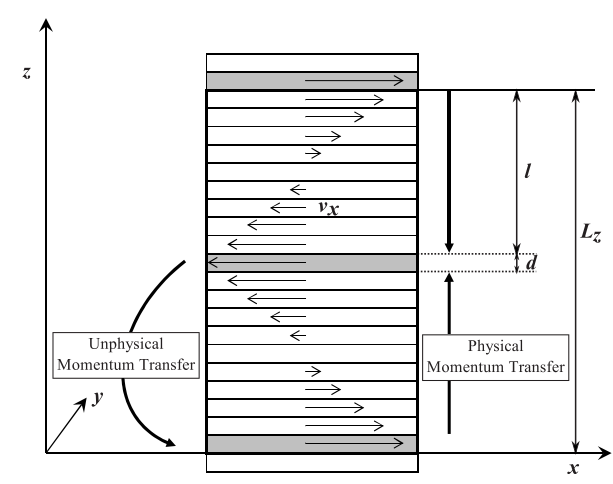
\includegraphics[width=0.4\textwidth]{figs/rnemd_box}%
	    	\caption{RNEMD Simulationsbox aus \cite{Tenney2010}, Fig. 1.}
   		\end{figure}		 
		 
	\end{itemize}
	
	\subsubsection{Strahlungsinduzierte Viskosität}
	Relaxation in Abhängigkeit von der Anzahl der Displacements.\\
	Ein biaxialer Stress ($\sigma_{xx} = \sigma_{yy}$, alle anderen Komponenten des Spannungstensors sind 0) wird eingebracht. Herleitung aus dem viskoelastischen Modell\cite{hobler2017hpm}
	\begin{equation}\label{eqn:visco1}
	   \pdv{\bm{\varepsilon}^{'} }{n_\mathrm{dpa} } = \frac{1}{2G} \pdv{ \bm{\sigma}^{'} }{n_\mathrm{dpa}} + \frac{1}{2\eta^{'} }  \bm{\sigma}^{'} 
	\end{equation}
	
	\begin{align}\label{eqn:visco2}
		p &= - B \varepsilon_\mathrm{V}\\
		-\frac{1}{3} \left(\sigma_{xy} + \sigma_{yy} + \sigma_{zz} \right) &= - B \left( \varepsilon_{xx} + \varepsilon_{yy} + \varepsilon_{zz} \right)
	\end{align}
	
	Da $\sigma_{xx} = \sigma_{yy}$ gilt, wird $\varepsilon_{xx} = \varepsilon_{yy}$ angenommen. Die deviatorischen Tensoren haben bezüglich der kartesischen Basis die Form
	\begin{equation}
	  \bm{\varepsilon}^{'}  = \begin{bmatrix}
    \varepsilon_{xx} - \frac{1}{3} \left( \varepsilon_{xx} + \varepsilon_{yy} + \varepsilon_{zz} \right)     & \varepsilon_{xy} & \varepsilon_{xz} \\
     \varepsilon_{xy} &  \varepsilon_{yy} - \frac{1}{3} \left( \varepsilon_{xx} + \varepsilon_{yy} + \varepsilon_{zz} \right)     &  \varepsilon_{yz}  \\
     \varepsilon_{xz} &  \varepsilon_{yz} &  \varepsilon_{zz} - \frac{1}{3} \left( \varepsilon_{xx} + \varepsilon_{yy} + \varepsilon_{zz} \right)    
\end{bmatrix}, 
	\end{equation}
	
		\begin{equation}
	  \bm{\sigma}^{'}  = \begin{bmatrix}
    \sigma_{xx} - \frac{1}{3} \left( \sigma_{xx} + \sigma_{yy} + \sigma_{zz} \right)     & \sigma_{xy} & \sigma_{xz} \\
     \sigma_{xy} &  \sigma_{yy} - \frac{1}{3} \left( \sigma_{xx} + \sigma_{yy} + \sigma_{zz} \right)     &  \sigma_{yz}  \\
     \sigma_{xz} &  \sigma_{yz} &  \sigma_{zz} - \frac{1}{3} \left( \sigma_{xx} + \sigma_{yy} + \sigma_{zz} \right)    
\end{bmatrix}.
	\end{equation}
	
	Mit eingesetzten Randbedingungen ergibt sich
	
	\begin{equation}
	  \bm{\varepsilon}^{'}  = \begin{bmatrix}
    \frac{1}{3} \left( \varepsilon_{xx} - \varepsilon_{zz} \right)     & \varepsilon_{xy} & \varepsilon_{xz} \\
     \varepsilon_{xy} &  \frac{1}{3} \left( \varepsilon_{xx} - \varepsilon_{zz} \right)     &  \varepsilon_{yz}  \\
     \varepsilon_{xz} &  \varepsilon_{yz} &  - \frac{2}{3} \left( \varepsilon_{xx} - \varepsilon_{zz} \right)
\end{bmatrix}, 
	\end{equation}
	
		\begin{equation}
	  \bm{\sigma}^{'}  = \begin{bmatrix}
     \frac{1}{3} \sigma_{xx}     & 0 & 0 \\
     0 & \frac{1}{3} \sigma_{xx}     & 0  \\
    0 &  0 &  - \frac{2}{3} \sigma_{xx} 
\end{bmatrix}.
	\end{equation}
	
	Aus \refeqn{eqn:visco1} folgt, dass alle Nicht-Diagonalelemente des Verzerrungstensors konstant bei eingebrachter Spannung bleiben. Die xx- und yy-Kompontente in \refeqn{eqn:visco1} ergeben diesselbe Differentialgleichung, während die zz-Komponente eine Linearkombination ist. Daher reduziert sich die tensorielle auf eine skalare Differentialgleichung
	\begin{equation}
	 \pdv{  \left(\frac{1}{3} \left( \varepsilon_{xx} - \varepsilon_{zz} \right) \right) }{n_\mathrm{dpa} } = \frac{1}{2G} \pdv{ \left( \frac{1}{3} \sigma_{xx} \right)}{n_\mathrm{dpa}} + \frac{1}{2\eta^{'} }  \frac{1}{3} \sigma_{xx}
	\end{equation}
	
    Die Normalspannung $\sigma_{xx}$ wird vorgegeben, daher ändert sie sich nicht, wenn displacements eingefügt werden.
    
    	\begin{equation}\label{eqn:scalar1}
	 \pdv{  \left(\frac{1}{3} \left( \varepsilon_{xx} - \varepsilon_{zz} \right) \right) }{n_\mathrm{dpa} } = \frac{1}{2\eta^{'} }  \frac{1}{3} \sigma_{xx}
	\end{equation}
	
	Die \refeqn{eqn:visco2} vereinfacht sich zu
	
	\begin{equation}\label{eqn:scalar2}
	  -\frac{2}{3} \sigma_{xx} = - B \left( 2 \varepsilon_{xx} + \varepsilon_{zz} \right).
	\end{equation}
	
	Wenn \refeqn{eqn:scalar2} in \refeqn{eqn:scalar1} eingesetzt wird, ergibt sich
	
	\begin{equation}
	  - \frac{1}{2} \pdv{  \varepsilon_{zz} }{n_\mathrm{dpa} } = \frac{1}{2\eta^{'} }  \frac{1}{3} \sigma_{xx}
	\end{equation}
	
	Daraus folgt der displacement-abhängige Verlauf der Dehnung in z-Richtung
	\begin{equation}
	  \boxed{ \varepsilon_{zz} = -  \frac{1}{3\eta^{'} }  \sigma_{xx} n_\mathrm{npa},}
	\end{equation}
 	
 	also eine lineare Abhängigkeit von $n_\mathrm{dpa}$.
	
	
\subsection{Gleichgewichts-MD Methoden (equilibrium MD, EMD)}
Dynamische Viskosität wird über Fluktuationen der \textbf{Nicht-Diagonalelementen des Spannungstensor} bestimmt. Die erhaltenen Wert gelten nur für \textbf{Newtonsche Fluide} ($\tau \propto \dot{\gamma}$). Prinzipiell sind die Ausdrücke nur im Grenzfall unendlich langer Simulationszeit und unendlich großer Simulationszelle gültig. Zusätzlich liegt typischerweise signifikantes thermisches Rauschen vor, was das SNR verringert. Daher ist eine große Zahl von Simulationsschritten nötig.\cite{Tenney2010}.

	\subsubsection{Autokorrelation des Spannungstensors (Green-Kubo)}
		\begin{itemize}
			 \item Green-Kubo-Relationen (Primärquellen: \cite{Green1954,Kubo1957}, Sekundärquellen für Viskositäts-Formulierung: \cite{Kirova2015,Tenney2010})
			 	\begin{equation}\label{eqn:green_kubo}
			 		\eta = \beta V \int_0^\infty \langle P_{xz}(0) P_{xz}(t) \rangle \mathrm{d} t 
				\end{equation}			 
				
				$\beta = 1/k_\mathrm{B} T$\\
				$V$ ... Volumen der Simulationsbox\\
				$P_{xz}$ ... xz-Komponente des Spannungstensors\\
				$\langle \ldots \rangle$ ... Ensemble-Mittelwert
			 
		 	\item Viskosität wird damit aus der \textbf{Autokorrelationsfunktion} der xz-Komponente des Spannungstensors $P_{xz}$ bestimmt
		 	\item xz-Komponente des Spannungstensors \cite{Kirova2015}
		 		\begin{equation}
					P_{xz} = \sum_{i=1}^N \frac{p_i^x p_i^z}{m_i} - \sum_{i>j}^N (x_i - x_j) \frac{\partial u_{ij} }{\partial z_j}	 	
			 	\end{equation}
			 	
			 	$p_i^{x,z}$ ... Komponente des Impulses des i-ten Teilchens\\ 
			 	$u_{ij}$ ... Interaktionspotential zwischen Teilchen j und Teilchen i\\
			 	$m_i$ ... Masse des i-ten Teilchens\\
			 	$x_i$ ... Ortsvektorkomponente von Teilchen i.
			 	
			\item Für \textbf{isotrope} Systeme existiert eine alternative Formulierung, die die Symmetrie ausnützt\cite{Tenney2010,Daivis1994}.
				\begin{equation}
					\eta = \frac{\beta V}{10} \int_0^\infty \langle P_{ij}^{os}(0) P_{ij}^{os}(t) \rangle \mathrm{d} t
				\end{equation}
			   
			    $P_{ij}^{os}$ ist eine Komponente des spurfreien symmetrischen Anteils des Spannungstensors.
			    \begin{equation}
			    	P_{ij}^{os} = \frac{P_{ij} + P_{ji} }{2} - \delta_{ij} \frac 1 3 \sum_k P_{kk}
			    \end{equation}
			    
    		 \item Setup der LAMMPS MD Simulationen von \cite{Kirova2015,Tenney2010} 
		 		\begin{itemize}
		 			\item 3D orthogonale Simulationsbox
		 			\item Periodische RB
		 			\item Verlet Zeitschrittverfahren
		 			\item Equilibrisierung bei \SI{20}{K} mithilfe eines Berendesen Thermostats (kein Impulstausch findet statt)
		 			\item Methode von \cite{Kirova2015}: MD Trajektorie wird in zeitliche Segmente eingeteilt und zeitliche Mittelung gemäß \refeqn{eqn:green_kubo} wird durch Ensemble-Mittelwert der einzelnen Segmente ersetzt.
		 		\end{itemize}
			 	
		 	\item Bsp in LAMMPS verweist auf \cite{Daivis1994}
		\end{itemize}

	\subsubsection{Einstein Formulierung}
		\begin{itemize}
			 \item Viskosität wird über einen Grenzwert aus der Fluktuation des Spannungstensors ermittelt \cite{Tenney2010}
			 
			 	\begin{equation}\label{eqn:tenney}
					\eta = \lim_{t\to\infty} \frac{\beta V}{2 t} \left\langle \int_0^t P_{xz}(t')\mathrm{d}t' \right\rangle
				\end{equation}
				
			 \item Kirova \cite{Kirova2015} verweist auf eine andere Formel, die bereits 1960 von Helfand \cite{Helfand1960} beschrieben wurde.
			    \begin{equation}\label{eqn:Kirova}
					\eta = \lim_{N,V,t\to\infty} \frac{\beta}{2 V t} \left\langle \left[\sum_{i=0}^N x_i(t) p_i^z(t) - \sum_{i=1}^N x_i(0) p_i^z(0) \right]^2 \right\rangle
				\end{equation}
				
				Diese hat eine ähnliche Form wie die bekannte Einstein Relation für die Diffusionskonstante
				\begin{equation}
					D = \frac{1}{6t} \left\langle \left[ \sum_{i=0}^N r_i(t) - r_i(0) \right]^2 \right\rangle
				\end{equation}
				
			\item Helfand \cite{Helfand1960} beschreibt allgemein, dass für kanonische Systeme, deren Zeitentwicklung von einem definierten Anfangszustand heraus betrachtet wird, ein Zusammenhang zwischen der Autokorrelationsformulierung und der Einstein'schen Form hergestellt werden kann. Unter gewissen Voraussetzungen (siehe  \cite{Helfand1960})  gilt
			
				\begin{equation}
					\langle (\Delta G)^2 \rangle = 2 t \int_0^\infty \langle J_0 J_\tau \rangle \mathrm{d} \tau,\quad J_\tau = \frac{ \mathrm{d} G }{\mathrm{d} \tau}
				\end{equation}
				
				Die Einstein'sche Formulierung gemäß \refeqn{eqn:Kirova} sollte damit prinzipiell \textbf{äquivalent} mit der Green-Kubo-Formulierung sein. \textit{Kann die Formulierung nach \refeqn{eqn:tenney} überhaupt stimmen?}
				
			 
			 \item Die prinzipielle Vorgangsweise bei der MD Simulation ist dieselbe wie bei der Green-Kubo-Methode.
		\end{itemize}

	\subsubsection{Abwandlung für die strahlungsinduzierte Viskosität}
	\textit{Ist es prinzipiell möglich mit Gleichgewichtsmethoden auf die strahlungsinduzierte Viskosität zu schließen?}

\section{Experimentelle Befunde}

\subsection{Stress und Viskositätsbetrachtungen}
	\begin{itemize}
		\item Betrachtungen für $\mathrm{SiO_2}$ in \cite{Snoeks2000}
		\item \textit{Wird der Begriff der strahlungsinduzierten Viskosität auch in der experimentellen Literatur verwendet?}
	\end{itemize}

\section{Simulation}

Als einzigen Vergleichswert für a-Si findet man in \cite{Vauth2007} $\eta(T=\SI{300}{K}) = \SI{9.656e8}{dpa}$.

\subsection{Erzeugen von a-Si aus c-Si}
	\begin{itemize}
		\item Gängige Methode zum Erzeugen von a-Si ist eine sogenannte \textit{Melt and Quench} Methode, bei der das kristalline Material geschmolzen und dann rapide abgekühlt wird.
		\item Meist wird ein \textbf{Berendsen Thermostat} mit \textbf{Stillinger-Weber} Potentialen verwendet (oder sehr rechenintensive ReaxFF - Potentiale)
		\item Erster Versuch mit ähnlichen Parametern wie bei der a-Ge Erzeugung in \cite{Mayr2005}.
		\item Verifizierung mit unterschiedlichen Kühlraten (Energie soll am Ende gleich bleiben? - TBD).
		\item In \cite{Vauth2007} wird a-Si aus flüssigem Si (mit \SI{6000}{K}), welches mit \SI{20}{Kps^{-1}} auf \SI{10}{K} gekühlt wird, erzeugt. Dabei wurden aber im Unterschied zu \cite{Mayr2005} Tersoff-Potentiale ausschließlich verwendet (eigentlich zu hoher Schmelzpunkt).
	\end{itemize}

\subsection{biaxiale Verzerrung}
	\begin{itemize}
		\item Verwenden des \texttt{fix deform} Kommandos, um die Simulationszelle gleich in x- und y-Richtung zu verformen.
		\item unterschiedliche Verformungen (in Vielfachen der Kantenlänge) geben unterschiedlich Startwerte für die biaxiale Spannung ($\sigma_{xx0}$) - evtl. mit Werten aus \cite{Mayr2005} und \cite{Mayr2003} ($\sigma_0 = \SI{1}{\giga\pascal}$) vergleichen.
	\end{itemize}

\subsection{Recoilgeneration}
	\begin{itemize}
		\item Verwenden des \texttt{velocity} Kommandos um \textbf{einem} zufällig ausgewählten Atom eine zufällige Geschwindigkeit zuzuweisen
		\item Vorschlag: Generieren der zufälligen Geschwindigkeitskomponenten in Python und schreiben der Variablen in .in File
		\item Größe der Simulationsbox muss abhängig sein von der eingebrachten Energie.
		\item Randbedingungen verwenden um Aufheizen zu vermeiden - vgl. Sputtern
	\end{itemize}

\bibliographystyle{Citation/IEEEbib-c.bst}
\bibliography{Citation/MolecularDynamics}


\end{document}  
